\chapter{Implementação do sistema proposto}
\label{cap:Implementacao}

% falta falar sobre filesystem vfs e como chegar ao socket file private\_data para alem da parte de interrupts, tasklets e bottomhalfs bem como sobre os contextos de execucao
%Falta falar sobre os motivos e a estrutura desejada para esta implementação



O principal desta dissertação consiste no desenvolvimento de um módulo do núcleo que consiga estender as funcionalidades do \textit{LSF} de forma a introduzir a funcionalidade de monitorização do tráfego realizado por um processo, tirando partido da instrumentação de código do núcleo.
O facto desta instrumentação ser efectuada no núcleo permite que qualquer aplicação possa ser monitorizada, sem que o seu código tenha de ser alterado.
Como se pode compreender, esta instrumentação é não instrusiva para as aplicações, havendo, deste modo a necessidade de criar uma método de verificação que identifique o processo que irá cada função instrumentada.
Esta adição ao \textit{LSF} irá conter um sistema externo, possibilitando a sua utilização sem a necessidade de modificar qualquer aplicação que tire partido da utilização do \textit{LSF}.
As modificações necessárias às extensões das funcionalidades do \textit{LSF} no núcleo estão confinadas ao ficheiro \textit{filter.c}, presente no directório \textit{net/core} do código do \textit{Linux}.

\section{MRoP e a sua implementação}
\label{sec:mrop_implementation}

A implementação da solução \textit{MRoP} teve em consideração o desenvolvimento de um código minimalista, que implicasse ligeiras alterações ao código do núcleo, e ao mesmo tempo, tirasse partido de \textit{APIs} internas.
É opaco à implementação da biblioteca \textit{PCap}, e pode ser integrado nesta.
A implementação está autocontida num módulo do núcleo, de modo a ser carregada e libertada, do mesmo, pelo administrador.
A modularização das diversas componentes, permite um desenvolvimento autónomo de cada subcomponente.

No capítulo \ref{cap:trabrelacionado} foram apresentados, a título exemplificativo (secção \ref{sect:instrumentacao_casos_linux}), alguns sistemas que permitem efectuar monitorização ou filtragem de pacotes, com a indicação de um processo.
O \textit{MRoP}, embora utilize o sistema de instrumentação do núcleo \textit{KProbes}, diferencia-se das soluções apresentadas, por se encontrar totalmente implementado no núcleo, com reduzida utilização de memória e perturbação do sistema.

Como apresentado na secção \ref{sub:network_cap}, o sistema de monitorização de rede é utilizado para cada pacote que passa pelo controlador de rede.

\begin{figure}[ht]
\centering
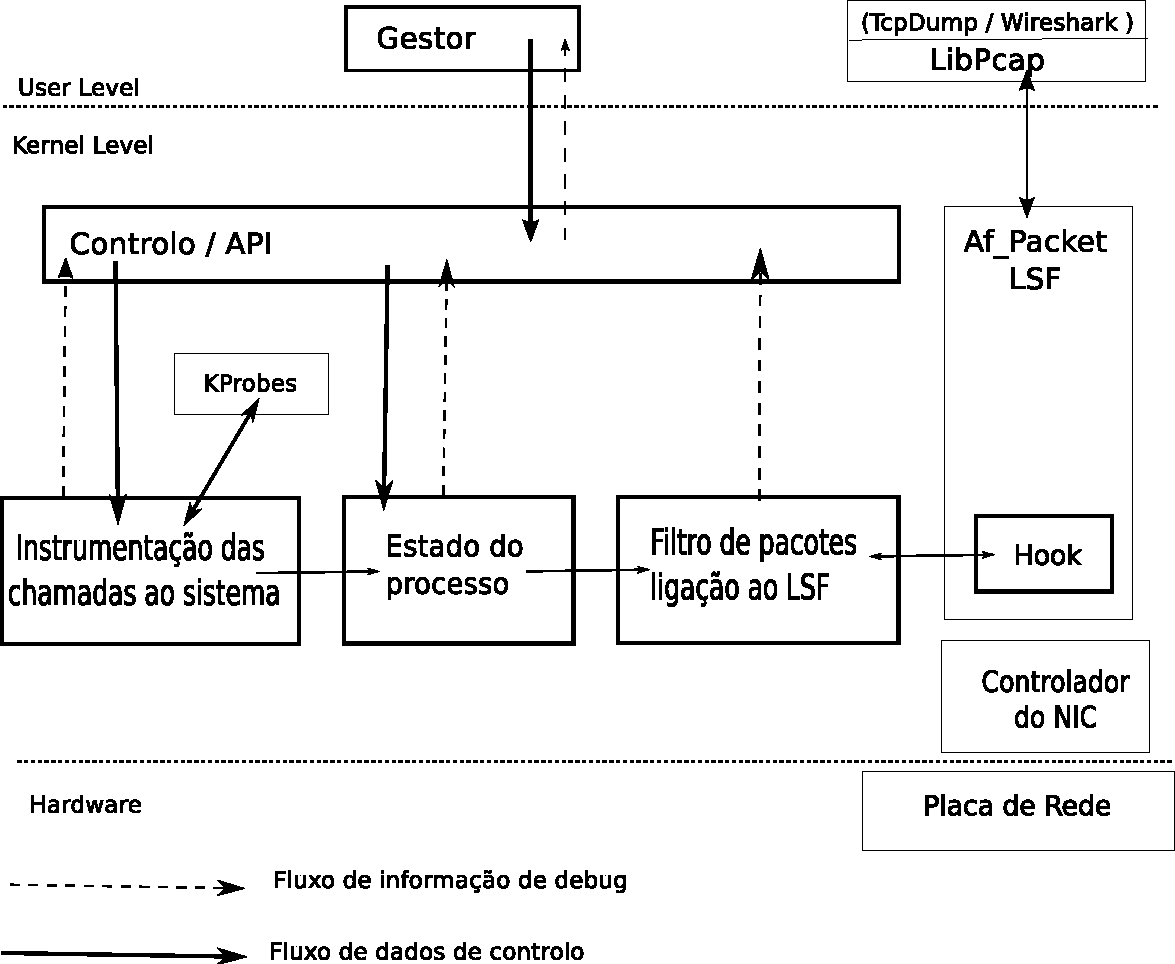
\includegraphics[scale=0.7]{arquitectura.pdf}
\caption{Arquitectura geral do MRoP}
\label{fig:general_architecture}
\end{figure}





%Por cada pacote ter de atravessar toda a arquitectura de rede incluida no \textit{vfs} seria demasiado pesado para o sistema.

%------- apresentar as diversas seccoes ao leitor ----------------

Nas subsecções seguintes irão ser apresentados os quatro componentes do \textit{MRoP} como se constanta na figura \ref{fig:general_architecture}.


\section{Instrumentação de funções do núcleo}

%----------------------------------------------------------------------------------------------------------

%Como foi anteriormente descrito em \ref{subsection:network} sobre as chamadas aos sistema para utilizar as funcionalidades de rede

%Foi necessário conhecer a \textit{ABI}\ref{ABI}\cite{ABI} referente às arquitecturas suportadas, \textit{x86} e \textit{x86\_64}, para a passagem de parâmetros das chamadas aos sistema.

%O sistema de \textit{KProbes} permite consultar os registos do processador onde foi efectuada a chamada à função (neste caso a chamada ao sistema).
% Por isso foram definidos 6 \textit{KRetProbes} referentes às chamadas \textit{connect}, \textit{bind}, \textit{accept}, \textit{sendto}, \textit{recvfrom} e
%\textit{close}.
% Para esta última \textit{close} devido à elevada utilização desta chamada ao sistema por diferentes aplicações no sistema, foi utilizada a função \textit{qqq coisa ...  ????}

%Para efectuar a monitorização das interacções de rede de um processo foi necessário recorrer à instrumentação de funções do núcleo.

%Através da instrumentação de funções do núcleo foi possível manter o contexto da execução do processo.

%Como apresentado e concluído na secção \ref{}, o sistema de monitorização que melhor se adequa ao problema exposto é o \textit{KProbes}.
% Deste sistema utilizou-se o \textit{KRetProbe}, de forma a instrumentar a entrada e retorno de funções.
% Obter os parâmetros de entrada das funções, principalmente o \textit{file descriptor}, tornou-se essencial.
% Para garantir que o repositório do estado do processo está coerente com o estado do núcleo, foi necessário obter o valor de retorno das funções.
% Por estas razões e porque as chamadas ao sistema têm ciclos de modificação da bastante lentos, o que evidência elevada estabilidade e consistência do núcleo, e por ser ponto de entrada do processo no núcleo foram as funções instrumentadas.

%As subsecções \ref{} .... \ref{} apresentam as funções do núcleo que foram instrumentadas.

%
% faltam as subsecoes ... 
%

%----------------------------------------------------------------------------------------------------------

A metodologia aplicada à resolução do problema de desempenho, baseia-se no desenvolvimento de uma componente para efectuar uma análise aos canais de comunicação de rede, utilizados por um processo, que insira a informação necessária no repositório.
Assim que um pacote chega ao sistema de monitorização, o \textit{LSF} tira partido do repositório para decidir a captura dos pacotes.


De entre os sistemas analisados o \textit{KProbes} foi aquele que permitiu obter menor sobrecarga, apesar do seu caracter dinâmico.
Os restantes contêm componentes de \textit{logging} que, para a realização deste estudo, apresentam uma sobrecarga desnecessária, afectando negativamente o desempenho.

Para além do sistema de instrumentação utilizado foi igualmente considerado o número de funções a instrumentar.
A sobrecarga total exercida pela instrumentação de funções do núcleo, tem em conta não só o número de funções que são instrumentadas, como o número de vezes que estas são executadas.

O conhecimento adquirido com a análise efectuada no capítulo \ref{cap:Estrutura}, sobre a \textit{Arquitectura de rede em Linux}, afectou positivamente a opção sobre as funções a instrumentar.

O \textit{MRoP}, foi desenvolvido para monitorizar a utilização de canais da familia \textit{INET}, tendo como particularidade, a utilização de canais baseados nos protocolos \textit{TCP} e \textit{UDP}, e instrumentar um número reduzido de funções do núcleo, pertencentes ao subsistema de rede.

O \textit{TCP} e o \textit{UDP} apresentam algumas funções em comum com protocolos de outras famílias, principalmente quando são executadas chamadas ao sistema, onde o nível de abstracção sobre estes protocolos é elevado.
Com o objectivo de diminuir o número de funções a instrumentar, optou-se pelas chamadas ao sistema, obtendo assim um maior nível de abstração e um controlo directo dos processos de nível utilizador.

As chamadas ao sistema instrumentadas correspondem: \textit{sendto}, \textit{recvfrom}, \textit{connect}, \textit{bind}, \textit{accept} e \textit{close}.
As análises inicialmente efectuadas demonstraram que apenas a chamada ao sistema \textit{close}, era demasiadas vezes executada, penalizando o desempenho global do sistema.
Esta situação radica no facto da chamada ao sistema \textit{close}, ser utilizada extensivamente para fechar canais, independentemente destes serem ficheiros, \textit{sockets}, \textit{pipes}, etc.
Para contornar esta dificuldade, foi necessário encontrar uma função que lidasse exclusivamente com o fecho de \textit{sockets}, de modo a reduzir a sobrecarga imposta pela instrumentação.


\subsection{Filtro de processos}

%------------------------------------------------------------------------------------------------

%A filtragem dos processos que efectuam as chamadas ao sistema de rede impôs um novo desafio.
% Se apenas filtrar as chamadas de um processo/pid seria apenas verificar se o pid é igual ao que se pretende é trivial e com baixa sobrecarga.
% Para um utilizador que queria analisar um processo, e não saiba qual dos fluxos do processo é responsável pela comunicação de rede, tornou-se complicado.

%Com esta abordagem ainda existe a possibilidade de não se obter todas as \textit{task} do processo, caso este tenha um àrvore com mais de 3 níveis, mas a sobrecarga sobre o sistema é inferior à situação de monitorização da criação de processos no sistema.
% Estes três identificadores foram escolhidos pois permitem identificar até 3 níveis da árvore de um processo.

%Seria bom colocar uma imagem de uma àrvore de processo .... 

%Os identificadores têm de ser escritos para os ficheiros respectivos no \textit{DebugFs}, que serão explicados na secção \ref{}.

%-----------------------------------------------------------------------------------------------------

O \textit{KProbes}, é um sistema de instrumentação do núcleo que não distingue entre que funções, não \textit{inline}, está a efectuar a instrumentação.
Não existindo suporte no \textit{KProbes} para filtrar o processo, que efectuou a chamada ao sistema, foi necessário desenvolver uma metodologia que permitisse reduzir a sobrecarga, quando a monitorização é realizada sobre um processo, que não o desejado.

%-------------------------

%Os objectivos referidos principais continuam a ser reduzida sobrecarga e actualização permanente do(s) processo(s) a monitorizar.
%Tendo estas caracteristicas como base algumas possibilidades foram tidas em consideração, onde o principal desafio foi conseguir manter a informação actualizada.

%--------------------------------------

No intuito de ultrapassar esta dificuldade, poder-se-ia ter recorrido à criação de um repositório com a informação sobre os identificadores dos processos a monitorizar, sendo necessário, uma vez mais, uma estrutura de suporte a este repositório, bem como funcionalidades de adição, remoção, actualização e consulta.
Este repositório teria de conter a estrutura genealógica do processo a monitorizar, assim como uma componente que actualizasse essa informação.
A actualização desta estrutura poderia ser efectuada através da instrumentação da chamada ao sistema \textit{fork} ou \textit{clone}.
Sempre que fossem invocadas as funções já referidas, seria efectuada uma consulta ao repositório e, a partir da informação obtida, este seria ou não, actualizado.
Esta possibilidade, ao contemplar a remoção de dados do repositório, necessitaria também de instrumentar a função de término de processos.

Considerando que a actualização dinâmica deste repositório, sem aplicar alterações no código do núcleo, afectaria negativamente o desempenho do sistema na sua totalidade.
Assim, optou-se por excluir esta alternativa em virtude da criação e destruição de processos puderem apresentar custos elevados.


Face a esta situação, optou-se por efectuar uma análise aos campos da estrutura (\textit{task\_struct}), o que permitiu compreender o modo como os identificadores dos processos se relacionam com os identificadores dos membros da árvore genealógica do processo.
Desta análise concluí-se que, os identificadores \textit{pid}, \textit{tid} e \textit{ppid} permitem, na grande maioria das aplicações, identificar toda a árvore genealógica.





\section{Estado dos \textit{sockets} do processo}

De modo a manter a informação relativa aos endereços e portos em utilização por uma aplicação, sem requer a consulta sobre os canais de rede, foi necessário criar um repositório de dados, que contivesse informações relevantes para as decisões do filtro de captura.
Neste repositório, existe a necessidade de ter funções de inserção, remoção e consulta, sendo que qualquer uma destas, deverá ser efectuada com celeridade, procurando estruturas que tenham uma complexidade temporal \textit{BigO}, \textit{O(1)} ou \textit{O(log n)}.

Assim, as estruturas de dados com suporte no núcleo, que permitem a criação de um repositório de dados, como o requerido, são:

%\subsection{Com suporte no núcleo}
%outro titulo alternativas disponíveis

\begin{description}

\item[BitMap - ]
%\subsubsection{Bitmap}

O recurso a um mapa de \textit{bits}, permite, de um modo bastante rápido e com uma reduzida utilização de memória, conhecer se um determinado porto está em utilização, por um determinado processo.
O núcleo do sistema possui suporte para o tratamento de mapas de \textit{bits}, ou seja, este verifica se um determinado \textit{bit}, num conjunto de memória, está ou não activo, podendo igualmente afectar um determinado \textit{bit} num conjunto de memória.
Embora este processo seja extremamente rápido, carece de modularidade, na medida em que apenas controla os portos, não dispondo de suporte para protocolos ou múltiplos endereços de rede.
 
----------------------------------------------------------------------------------------------------------

Uma solução seria agrupar os diferentes mapas de bits sob a terminologia de um endereço, mas e se fosse udp ou tcp ?
E quando um processo efectua um bind sob todas as interfaces do sistema ? 
E quando é utilizada mais uma interface virtual sob uma real ? .....

----------------------------------------------------------------------------------------------------------

\item[Listas - ]

No núcleo existe uma implementação bastante eficiente da estrutura de dados \emph{lista} (\emph{list}), contendo apenas dois apontadores, destinando-se um ao elemento que o precede e outro ao que se lhe segue.

Embora não seja necessário definir uma lista com o máximo número de portos, dado que estes podem ser adicionados dinamicamente, a complexidade temporal de pesquisa no, pior caso é de \textit{O(n)} (traduzindo-se num mau indicador de desempenho para o estudo pretendido nesta dissertação).
No entanto quando o número de elementos não é elevado, a utilização de uma lista apresenta-se como uma boa solução.

%\subsubsection{Listas duplamente ligadas}
%\subsubsection{Árvores}

%\item[Árvores Binária - ]
%\todo{ver}
%Apesar de não ser necessário percorrer os elementos ou obter os indíces de forma ordenada. 

%\paragraph{Arvores Balanceadas}
\item[Árvore Balanceada- ]
\textit{Red-black Tree} 

No núcleo existe uma implementação parcial de uma árvore \textit{Red-black} genérica, a fim de permitir o acesso aos dados através de chaves, ou seja, trata-se de uma estrutura associativa.%\cite{}
A árvore \textit{Red-black} é semi-balanceada, isto é, a diferença de alturas entre o ramo mais profundo e o mais curto é de apenas de nível 1.
Esta propriedade é mantida através do rebalanceamento da árvore em inserções e remoções, o que provoca um custo na sua utilização.
Contudo no caso esperado, existe maior número de consultas do que inserções e remoções, o custo associado ao rebalanciamento da árvore é amortizado.
De modo a tirar partido da utilização desta estrutura de dados é necessário definir três funções da manipulação da árvore (inserção, remoção e consulta).
O suporte disponibilizado pelo núcleo apenas permite manusear a árvore, sendo necessário definir as funções que utilizam a chave de acesso para aceder ao conteúdo dos dados, que devido à sua especificidade, não foram incluídas no suporte.

De referir igualmente, que para o objecto deste estudo, o número do porto dos protocolos (\textit{TCP} e \textit{UDP}), é considerada a chave mais adequada.
Considerando o número máximo de portos possíveis nos protocolos (\textit{TCP} e \textit{UDP}), a árvore terá de conter 65535 elementos, com uma altura máxima de 16, ou seja, para pesquisar um dos elementos nos extremos (máximo ou mínimo) é necessário efectuar sobre ela, 16 iterações.
Embora não constitua um requisito, é possível obter de forma ordenada todas as chaves, bem como os valores que lhe estão associados.

-----------------------------------------------------------------------------------------------------------

Complexidade de inserção, pesquisa e remoção é O(log n), sendo n o número de elementos da árvore.

Pode existir uma penalização no desempenho, devido à necessidade de balancear a àrvore.
Os ganhos provenientes deste balanceamento, face às àrvores não balanceadas, permite manter a complexidade média de acesso aos dados em O(log(n)), ao invés de um possível decremento até O(n), ou seja a árvore degenerar numa lista.

-----------------------------------------------------------------------------------------------------------

%\item[Radix Tree - ]
%talvez falar sobre esta arvore ....

\end{description}

\paragraph*{}
Outras estruturas de dados passíveis de serem consideradas, apesar de não possuirem suporte no núcleo.

\begin{description}
%\subsubsection{Tabela de dispersão}
\item[Tabela de Dispersão]
No núcleo existe uma implementação de tabelas de dispersão que efectuam a dispersão e o controlo sobre as suas chaves.

\end{description}
\paragraph*{}
A opção pela estrutura de dados \textit{Red-black tree} deve-se principalmente ao desempenho e à existência de implementação da estrutura no núcleo do \textit{Linux}.

O ciclo de desenvolvimento do \textit{MRoP}, foi efectuado mais rapidamente, tendo em consideração a confiança na validação da estrutura de dados \textit{Red-black tree}, uma vez que esta está em utilização no núcleo do sistema \textit{Linux} e tem sido sujeita a uma análise extensiva ao longo dos anos.
 
\subsection{Estrutura utilizada}
\label{sub:repo_structure}

Os elementos do repositório criado, através de uma árvore \textit{Red and Black}, têm uma estrutura bem definida, contendo obrigatoriamente um \textit{rb\_node}, para possibilitar a manipulação da árvore e um outro elemento, de carácter comparativo, utilizado como chave.

Além dos referidos, esta estrutura contempla outros elementos que seguidamente se descrevem:

\begin{figure}[ht]
\begin{minipage}[b]{0.5\linewidth}
\centering
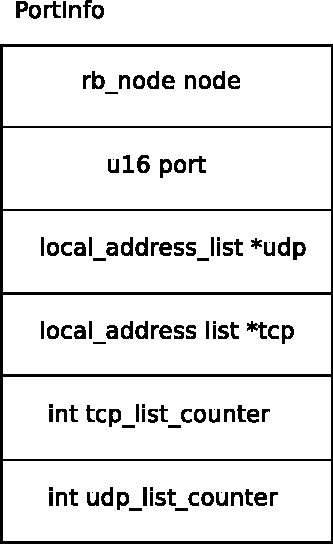
\includegraphics[scale=0.8]{portInfo_structure.pdf}
\caption{Elemento da árvore}
\label{fig:portInfo}
\end{minipage}
\hspace{0.5cm}
\begin{minipage}[b]{0.5\linewidth}
\centering

\includegraphics[scale=0.8]{local_address_list}
\caption{Lista de endereços}
\label{fig:local_address_list}
\end{minipage}
\end{figure}

A figura \ref{fig:portInfo} apresenta a disposição dos elementos da estrutura \textit{PortInfo}, sendo que as listas de endereços \textit{IP} das interfaces de rede, são adicionadas através na estrutura apresentada na figura \ref{fig:local_address_list}.
Os elementos do repositório, correspondem a instâncias da estrutura \textit{PortInfo}, aos quais são adicionados através dos \textit{handlers} das funções instrumentadas, em conformidade com o esquema apresentado na figura \ref{fig:repo_example}.

\begin{figure}[ht]
\centering
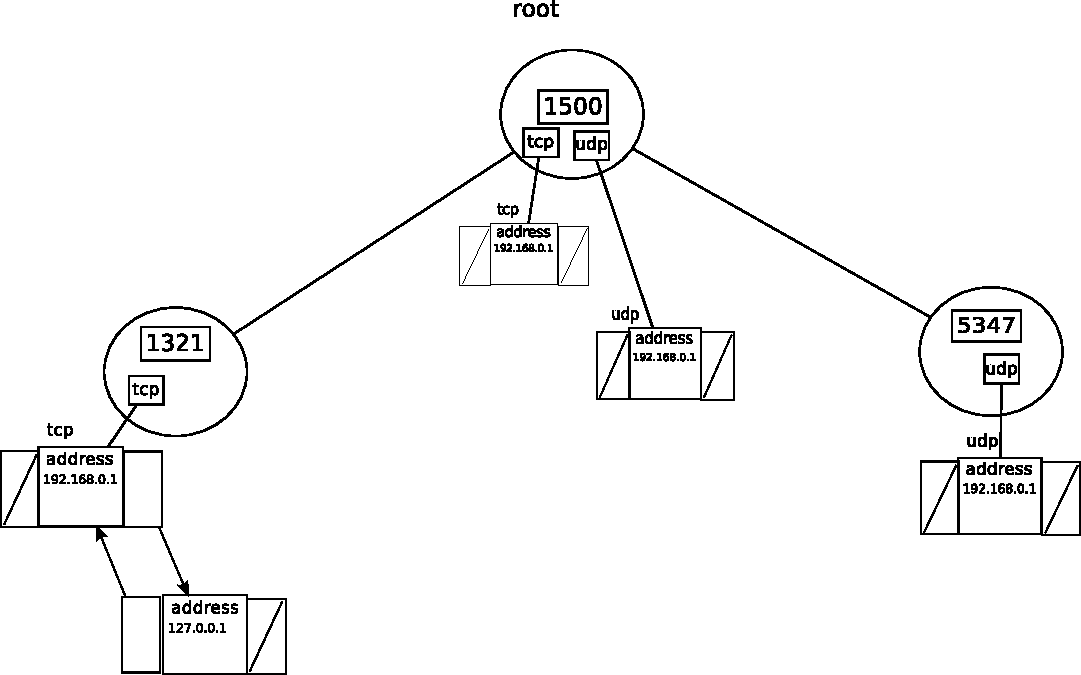
\includegraphics[scale=0.7]{repositorio_exemplo.pdf}
\caption{exemplo do repositório, Estado do Processo, com 3 portos}
\label{fig:repo_example}
\end{figure}

\subsection{\textit{API} de comunicação interna do MRoP}
\label{sub:repo_api}

Com o objectivo de efectuar inserções, consultas e remoções dos dados do repositório, foi desenvolvida uma \textit{API} interna ao \textit{MRoP}, que permite validar os parâmetros passados às funções do repositório de dados.
Através desta \textit{API} foi possível realizar a separação das componentes do \textit{MRoP} beneficiando, deste modo, a modularidade do código.

\begin{figure}[ht]
\centering
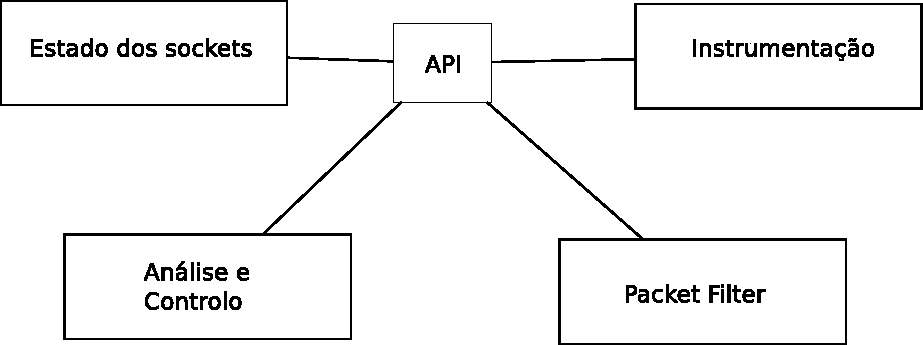
\includegraphics[scale=0.7]{API_connect_drawing.pdf}
\caption{API interna do MRoP}
\label{fig:api_connect}
\end{figure}

Esta \textit{API} permite aos \textit{handlers} das funções instrumentadas, efectuar as operações de inserção e remoção sobre a componente \textit{Estado dos Sockets}.
Relativamente à operação de consulta, esta é particularmente importante, na medida em que executa a filtragem de pacotes das interfaces de rede.

A \textit{API} não obstante, reduzir o desempenho, devido à necessidade de chamar os métodos específicos ao repositório, permite a substituição deste, sem que se verifique alterações do código.

Apesar dos processos monitorizados apresentarem elevado dinamismo nas interacções das comunicações, a maior percentagem de operações sobre o repositório concentra-se ao nível da consulta.
As restantes operações (inserção e remoção) repartem entre si igual percentagem.
Assim, é esperado que para cada inserção exista uma remoção.
No final da monitorização de um processo a componente \textit{Estado dos Sockets}, deverá apresentar um número de elementos identico ao que antecedeu a monitorização.


%\subsubsection{Identificadores}

%No núcleo do \textit{Linux} quando um processo é criado os identificadores, \textit{pid} e \textit{tgid} são iguais.

\section{Filtro de pacotes, extensão ao LSF}

No sistema de monitorização de rede, um dos componentes corresponde a uma função que serve de máquina virtual às instruções do \textit{LSF}.
Esta função itera sobre o filtro, executando instrução a instrução, sobre o pacote (recebido ou enviado), até ao momento em que identifica uma das instrução de retorno (\textit{BPF\_RET} ou \textit{BPF\_RET\_A}).
Consoante o valor retornado nestas instruções, o pacote analisado é, ou não, capturado.
Caso seja capturado, é efectuado um clone do pacote e colocado num \textit{ring buffer}, partilhado com a aplicação monitora de rede em nível utilizador.
Caso o valor retornado não corresponda a uma captura, a computação sobre esse pacote termina, reduzindo a sobrecarga da monitorização.
Assim, o facto de se tirar partido da utilização de um filtro, que identifique de forma célere a rejeição de um pacote, diminui consideravelmente a sobrecarga imposta ao sistema por parte da monitorização.

Face aos benefícios obtidos pela utilização do filtro, considera-se que o sistema de instrumentação do núcleo (\textit{KProbes}), poderia ser utilizado para invocar o novo sistema de filtragem criado e modificar o valor de retorno, caso se tornasse necessário.
Todavia, face ao número de vezes que a função de filtragem é invocada (uma para cada pacote, recebido ou enviado), a sobrecarga da utilização do \textit{KProbes} é de todo desaconselhável.

Assim, foi necessário modificar o código do \textit{Linux} de modo a inserir um \textit{hook}, ou seja um apontador para uma função, que será invocada quando o filtro estático for avaliado para captura, permitindo que a função \textit{MRoP} executado, permitindo assim efectuar uma conjunção entre o filtro estático definido pelo administrador e a filtragem dinâmica efectuada pelo \textit{MRoP}.

Assim, além da definição de um \textit{hook} para activação e desactivação deste novo sistema, foi efectuada uma alteração ao código do \textit{Linux} na função \textit{sk\_run\_filter}, que se traduziu no retorno da decisão conjunta do filtro estático com o dinâmico, ambas realizadas no ficheiro \textit{filter.c}.

Esta alteração permitiu adicionar uma nova funcionalidade, não obstante se assistir a uma ligeira sobrecarga no sistema de monitorização, independentemente da mesma estar ou não activa.

\begin{figure}[!ht]
\centering
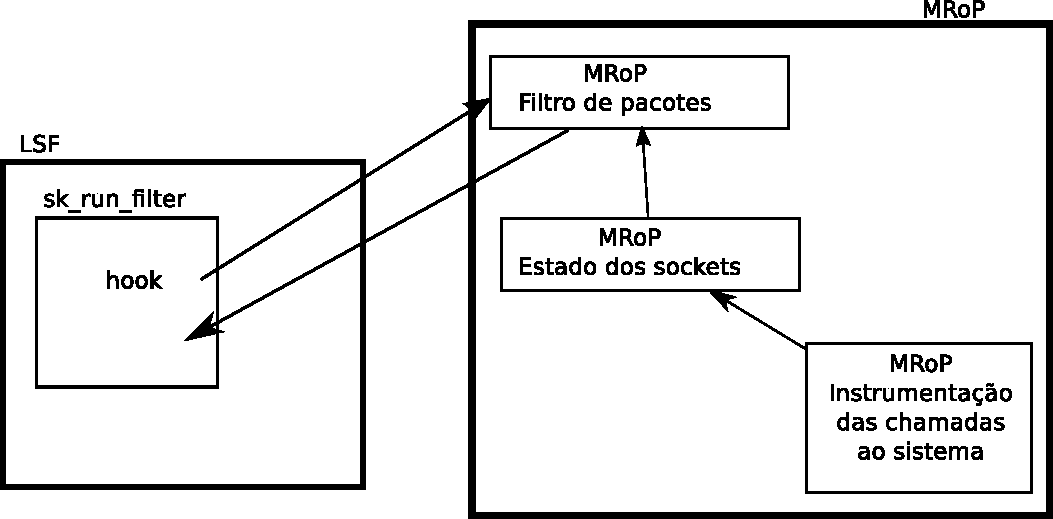
\includegraphics[scale=0.7]{run_filter.pdf}
\caption{Execução da nova filtragem de pacotes pelo LSF}
\label{fig:run_filter}
\end{figure}

%Para se poder definir uma nova instrução no \textit{Instruction Set}, é necessário alterar o ficheiro \textit{grammar.y}, na entrada correspondente à posição que deverá ocupar na \textit{AST (Abstract Sintax Tree)}, e modificar as funções de criação do novo filtro, quer em modo utilizador quer dentro do núcleo de sistema.
%Este desenvolvimento tem de ser realizado par-a-par, pois a ser efectuado apenas de um lado, o outro tornar-se-á incompatível.




\section{Informação de análise e controlo}

O \textit{MRoP} foi desenhado e implementado de modo a ser relativamente autónomo, apenas necessitando da configuração de alguns parâmetros, essenciais ao seu funcionamento.

Com o propósito de obter informações sobre o estado da computação dos diversos componentes da ferramenta e de invocar a monitorização, procedeu-se à criação de alguns ficheiros no \textit{DebugFs}, assim no que se refere à componente \textit{Informação de análise e controlo}, esta fica responsável pelos diversos aspectos da instrumentação e do repositório.

\subsection{Informação de controlo}

Os ficheiros de controlo criados foram: \textit{pid}, \textit{ppid}, \textit{tgid} e \textit{option}.
Estes ficheiros à excepção do último, são ficheiros que podem ser lidos e escritos pelo administrador, que caso já tenham sido escritos contêm o identificador respectivo do processo a monitorizar.
Caso não tenham sido escritos o valor por omissão é 0.
O ficheiro \textit{option}, tem apenas a permissão de escrita, e dependendo do valor escrito, pode activar a procura de portos no processo indicado em \textit{pid}, apagar todos os dados do repositório, e activar ou desactivar o filtro dinâmico.

\subsection{Informação de análise}
A informação de análise apenas é adicionada, caso o seu suporte seja activado na compilação, permitindo assim obter estatisticas sobre os diferentes componentes internos ao \textit{MRoP}.

Os ficheiros de análise apenas estão disponíveis para leitura, por isso quando lidos devolvem os valores presentes nos contadores internos do \textit{MRoP}.
Sobre os filtros estes contadores têm o número de pacotes que passaram no filtro dinâmico, bem como o número de pacotes que foram declarados para captura.
Em relação à monitorização do processo, existe também um ficheiro de devolve, em relação a cada uma das funções instrumentadas, o número de vezes que foi executado o \textit{handler} e quantas destas pertenciam ao processo alvo.
Para o repositório de dados foi também criado um ficheiro com estatisticas, estas incidiram sobre o número de portos em utilização, e para cada porto a indicação se esse porto está em utilização através do protocolo \textit{TCP}, \textit{UDP} ou em ambos, e por que endereço(s) de rede.

%\begin{figure}[ht]
%\centering
%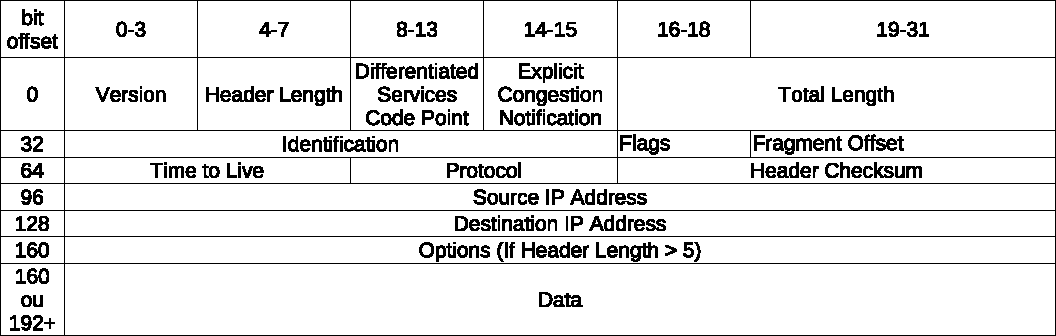
\includegraphics{Ipv4_table.pdf}
%\caption{Protocolo IPv4}
%\label{fig:ipv4_proto}
%\end{figure}


%\begin{figure}[ht]
%\centering
%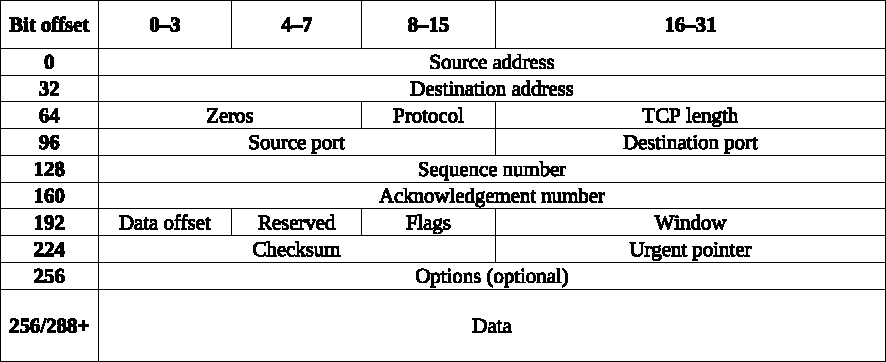
\includegraphics{tcp_table.pdf}
%\caption{Protocolo TCP em IPv4}
%\label{fig:ipv4_tcp_proto}
%\end{figure}

%\begin{figure}[ht]
%\centering
%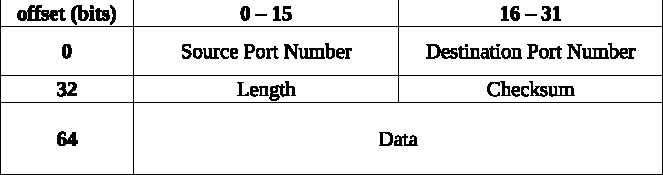
\includegraphics{udp_table.pdf}
%\caption{Protocolo UDP em IPv4}
%\label{fig:ipv4_udp_proto}
%\end{figure}


%\begin{figure}[ht]
%\centering
%url = http://upload.wikimedia.org/wikipedia/commons/3/3b/UDP_encapsulation.svg
%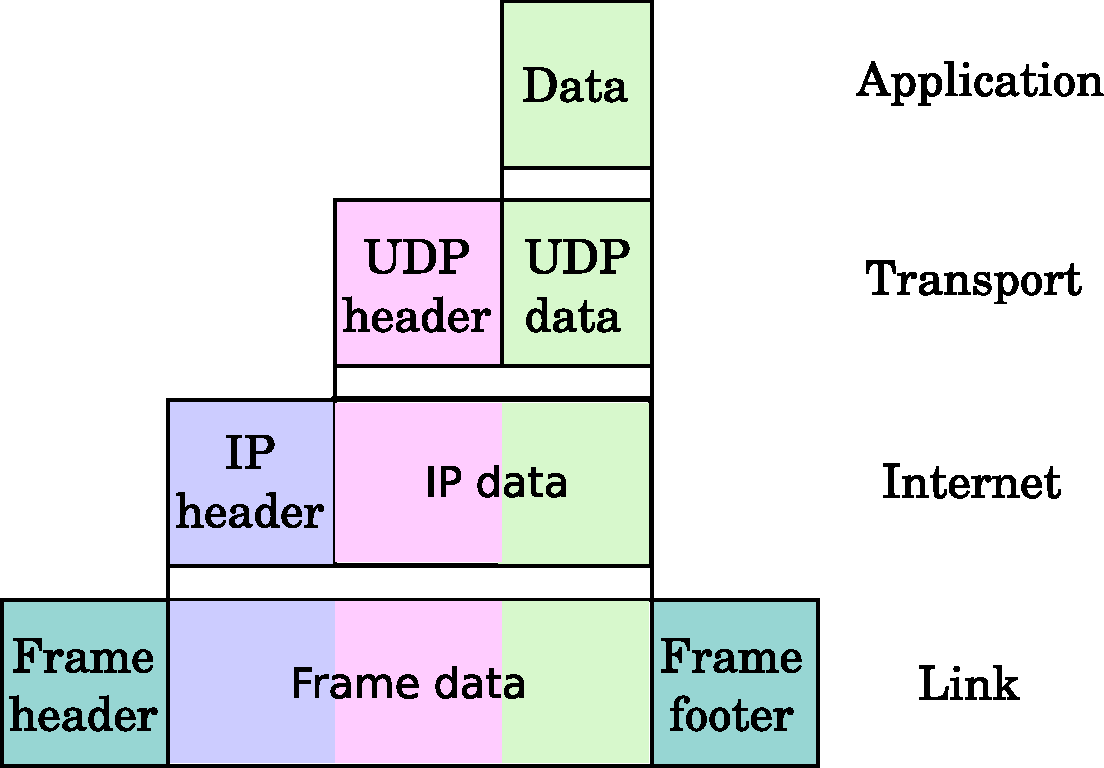
\includegraphics[scale=0.7]{UDP_encapsulation.pdf}
%\caption{Execução de filtragem de pacotes}
%\label{fig:run_filter}
%\end{figure}

%Quando o módulo da ferramenta é executado os indicadores de \textit{pid}, \textit{ppid} e \textit{tgid} são inicializados com o valor -1.

%Esta ferramenta de monitorização só irá passar a analisar os dados das chamadas ao sistema quando estes valores estiverem definidos e identificarem o processo que efectuou a chamada.

%\subsubsection{Sistema de Ficheiros}

%Dentro do sistema de ficheiros onde os \textit{sockets} estão incorporados, como apenas estamos interessados em analisar os sockets construidos para a familia \textit{AF\_INET} todos os sockets que não pertencerem a esta familia e não forem do tipo \textit{TCP} ou \textit{UDP} não serão mais analisados.
% Os \textit{sockets} que pertencem é então inicializado uma estrutura do tipo \textit{não me lembro ??? ver código} onde estão definidos o porto, o endereço e se são do tipo \textit{UDP} ou \textit{TCP}.

%Dependendo da chamada ao sistema realizada entre a função definida na entrada e a definida no retorno do \textit{KRetProbe}, são passados parâmetros que irão ser utilizados na função de retorno.


%\subsection{DebugFs}
%Criação de alguns ficheiros no sistema virtual \textit{configFs} para poder observar o comportamento da monitorização e dos pacotes que chegaram ao sistema de filtragem.
%A forte restrição de apenas um valor por ficheiro do \textit{SysFs} obriga a que para obter diferentes valores do sistema tenha de abrir diferentes ficheiros.
% Como o sistema de ficheiros \textit{proc} se sitia principalmente para os processos seria um bom candidado para a colocação de informação sobre 


%\section{Dificuldades}
% As chamadas ao sistema para o protocolo \textit{UDP} podem ser dificeis de analisar pois apesar de para o \textit{sendto} poder user utilizada a mesma técnica que foi utilizada para o \textit{connect}, para o \textit{recvfrom} pode ser mais dificil pois pode receber pacotes de multiplas fontes

\section{Conclusão}
\label{sec:implement_conclusion}
